

%\begin{itemize} 
%\item{ }
%A brief textual description of the overall flow diagram (along with its functional operation in the different user scenarios described in the first stage of the project).
%\item{ }
%A specification of each algorithm and associated data structures together with its entities, attributes, and operations ( include an English description of how they relate to your user scenario(s)).

%\end{itemize}

\begin{itemize} 
\item{  Short Textual Project Description. }
The recommendation system works along with users' inputs to give suggestions as a feedback to users about users' houses' prices. We build the system database using crawling, and deposit user's information to the database so that the recommendation system can calculate users' houses to new variables. The feedback includes prediction on house's price, recommended selling price. It is the same to other types of users. For example, landlords can decide when to sell the house for the maximum profit.
\item{ Flow Diagram: see Fig 1}
\begin{figure}
\centering
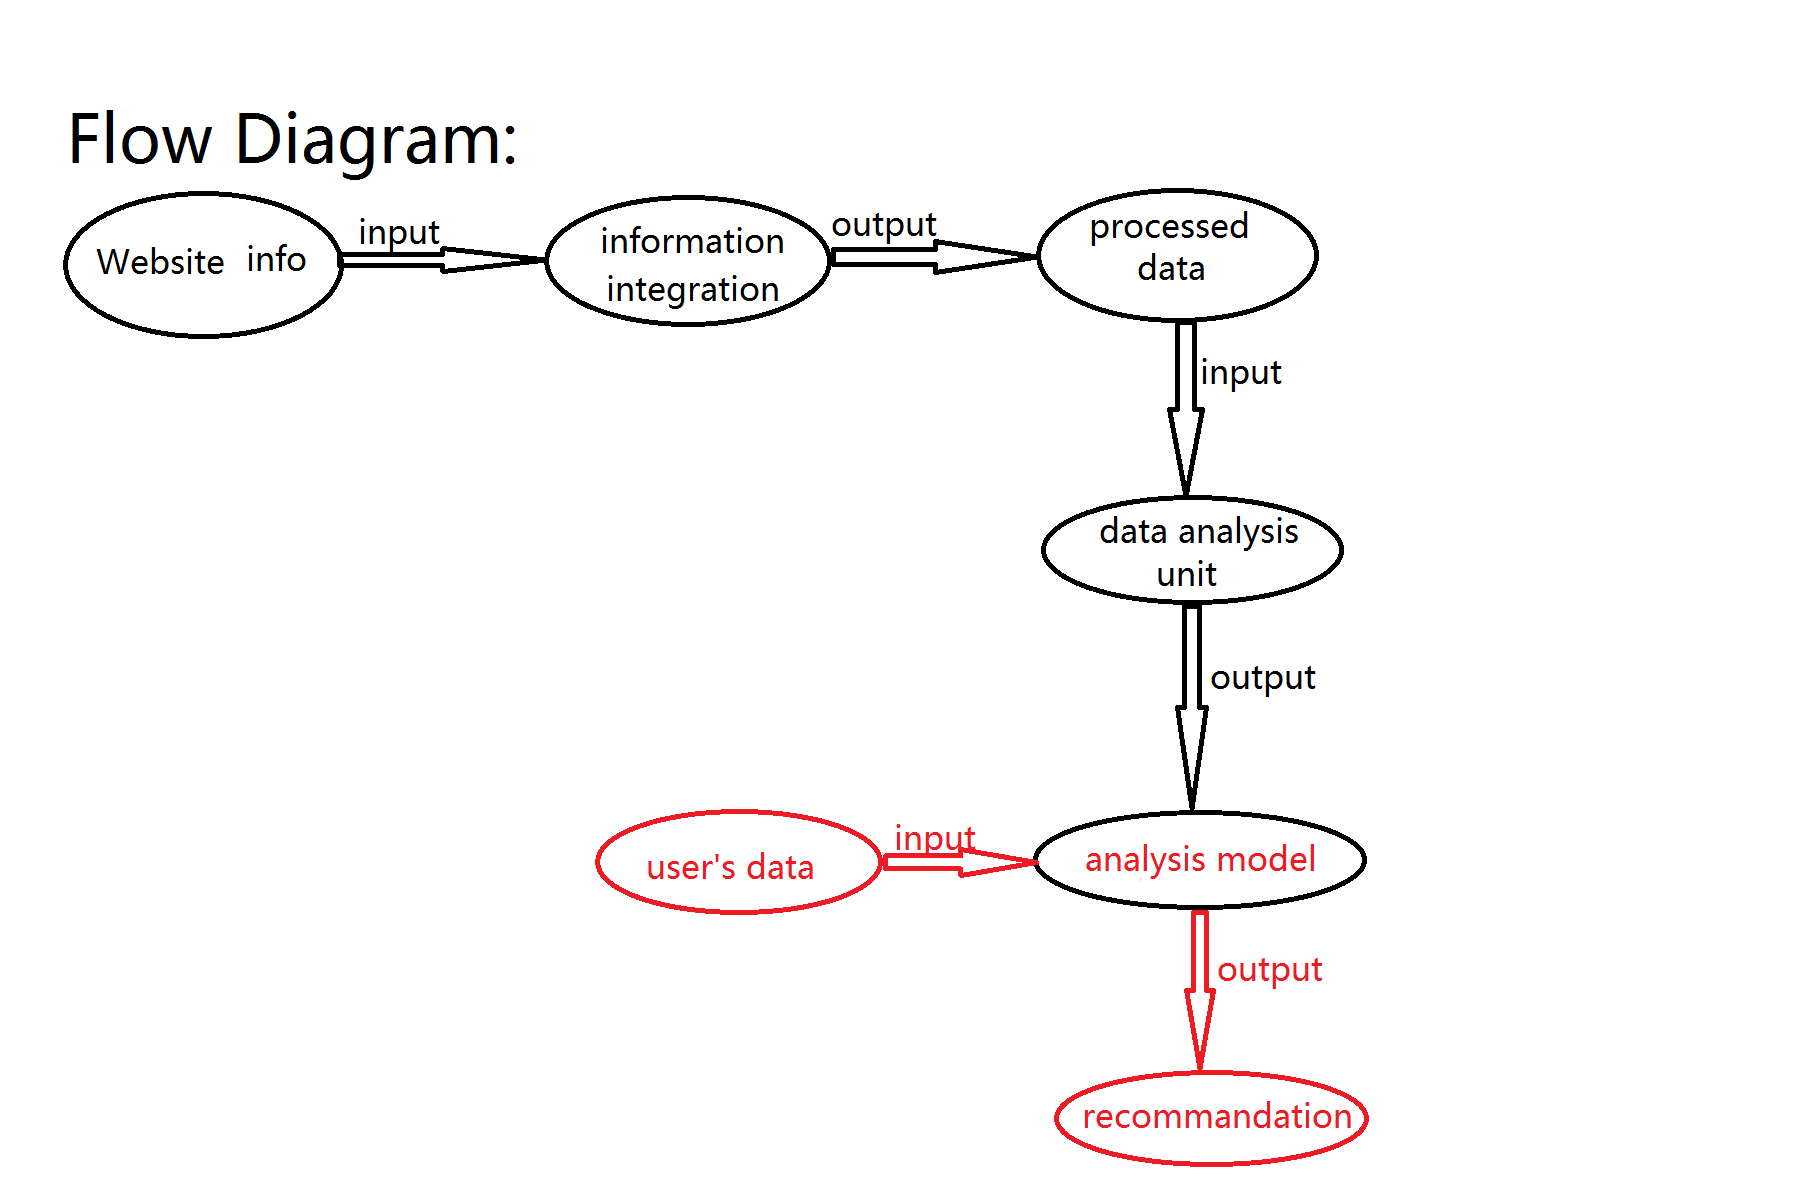
\includegraphics[width=0.4\textwidth]{512flowdiagram.png}
\caption{}
\end{figure}
\item{ High Level Pseudo Code System Description. }
\begin{itemize} 
\item{Information Integration Module: Integrating Unit(website-info)
We collect the houses' information of New Jersey from the website "weichert" using crawling to obtain the property information. Then we save the information to Excel files.
Return Processed data}

\item{Data Analysis Module: Data Analysis Unit(Processed data)
Pass Processed data to Data Analysis Unit, then process it through Regression Unit. The process procedure includes to uniform the file style, to remove the redundant information from the original dataset, to transform the non-digital information to digital information.
Deposit it to system database}

\item{User's Preference input()
Input User's preference}

\item{Regression Unit()
Rate user's input house, then give the prediction using linear regression on house's price. 
Form a suggestion feedback to users}
\end{itemize}
\item{Algorithms and  Data Structures. }
Algorithms and  Data Structures: First we use web crawling algorithm to stretch useful data from website. This algorithm works with website code and get different digital data from website. Secondly we process these data to table structure type which our data analysis unit could use. Finally, we use our model deal with digital data and output useful recommendations. 
\item{As to the data structure, we use list to save houses' information from the website, process the data using string, use data frame to achieve regression and price prediction.}
\item{The main algorithms used in our project are crawling to get the total information from the website, bubble sort which is used for sorting the house list according to the prices provided from the website and regression which is used for providing the standard of price prediction and providing similar houses from the system data-list.}
\end{itemize}

\begin{itemize} 
\item{  Flow Diagram Major Constraints.}

\begin{itemize} 
\item{ First integrity constraint: Houses data on the website must contain price, room numbers, year, area. }
\item{ Second integrity constraint: Input data to the data analysis unit must be table format with numbers. }
\end{itemize}
\end{itemize}
}
